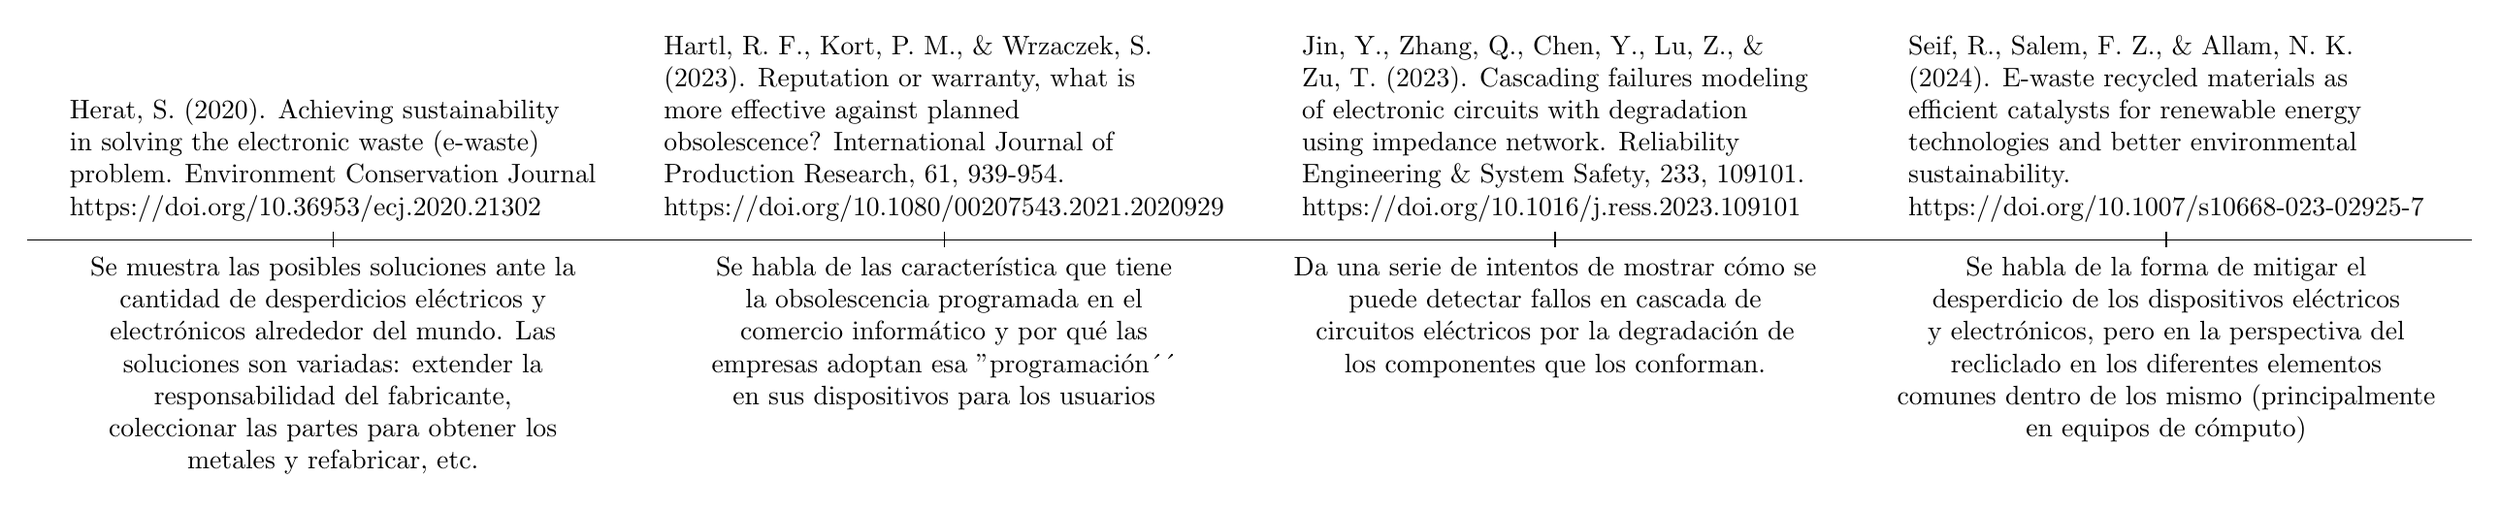
\begin{tikzpicture}
% draw a horizontal line
\draw (0,0) -- (32,0);
% draw vertical lines
\foreach \x in {4,12,20,28}
\draw (\x cm,3pt) -- (\x cm,-3pt);

% draw nodes to add events
\draw (4,0) node[below=3pt, align=center] {
  Se muestra las posibles soluciones ante la\\
  cantidad de desperdicios eléctricos y\\
  electrónicos alrededor del mundo. Las\\
  soluciones son variadas: extender la\\
  responsabilidad del fabricante,\\
  coleccionar las partes para obtener los\\
  metales y refabricar, etc.
} 
node[above=3pt, align=left] {
  Herat, S. (2020). Achieving sustainability\\
  in solving the electronic waste (e-waste)\\
  problem. Environment Conservation Journal\\
  https://doi.org/10.36953/ecj.2020.21302
};
\draw (12,0) node[below=3pt, align=center] {
  Se habla de las característica que tiene \\
  la obsolescencia programada en el \\
  comercio informático y por qué las \\
  empresas adoptan esa ''programación´´ \\
  en sus dispositivos para los usuarios \\
} node[above=3pt, align=left] {
  Hartl, R. F., Kort, P. M., \& Wrzaczek, S.\\
  (2023). Reputation or warranty, what is\\
  more effective against planned\\
  obsolescence? International Journal of\\
  Production Research, 61, 939-954.\\
  https://doi.org/10.1080/00207543.2021.2020929
};
\draw (20,0) node[below=3pt, align=center] {
  Da una serie de intentos de mostrar cómo se \\
  puede detectar fallos en cascada de \\
  circuitos eléctricos por la degradación de \\
  los componentes que los conforman.
} node[above=3pt, align=left] {
  Jin, Y., Zhang, Q., Chen, Y., Lu, Z., \&\\
  Zu, T. (2023). Cascading failures modeling\\
  of electronic circuits with degradation\\
  using impedance network. Reliability\\
  Engineering \& System Safety, 233, 109101.\\
  https://doi.org/10.1016/j.ress.2023.109101
};
\draw (28,0) node[below=3pt, align=center] {
  Se habla de la forma de mitigar el \\
  desperdicio de los dispositivos eléctricos \\
  y electrónicos, pero en la perspectiva del \\
  recliclado en los diferentes elementos \\
  comunes dentro de los mismo (principalmente \\
  en equipos de cómputo)
} node[above=3pt, align=left] {
  Seif, R., Salem, F. Z., \& Allam, N. K.\\
  (2024). E-waste recycled materials as\\
  efficient catalysts for renewable energy\\
  technologies and better environmental\\
  sustainability.\\
  https://doi.org/10.1007/s10668-023-02925-7
};
\end{tikzpicture}
